

\def \currentAuthor {Lukas Vogel} %so kann jederzeit der Autor geändert werden -> wird in der Fusszeile angezeigt.



\chapter*{Notationen}
Beschreibung wie Code, Hinweise, Zitate etc. formatiert werden  

\chapter{Einleitung}
Diese Diplomarbeit befasst sich mit der Entwicklung des Prototyps: NeXt. Das Produkt ist eine spielbare Version eines Computerspiels in dem sogenannte Jump and Run-Elemente, Puzzele-Elemente sowie Zeitmanagement-Elemente beinhaltet sind. Das Projekt wurde in Verbindung mit der Firma ClockStone Softwareentwicklung GmbH. erarbeitet. Interesse könnte diese Dokumentation bei jedem erwecken,	 der sich über Spielentwicklung in Verbindung mit der Unity-Engine  informieren will. Des Weiteren werden auch die Aspekte des Projektmanagements dieser Arbeit dargelegt.  

\chapter{Projektmanagement}

\section{Metainformationen}
\subsection{Team}

	\begin{figure}[H]
	\centering
		
\includegraphics[width=4cm]{images/LukasVogel.png}
		\caption{Lukas Vogel}		
	\end{figure}

	\textbf{Name:} Lukas Vogel\\
\textbf{Funktion:} Projekt Leiter\\
\textbf{Wohnort:} Hohenems\\
\textbf{E-Mail:} lvogel@tsn.at\\
\textbf{Aufgabenbereiche:} \begin{itemize}
	\item GUI
	\item Leveldesign
	\item Dokumentation
\end{itemize}
\begin{figure}[H]
	\centering
	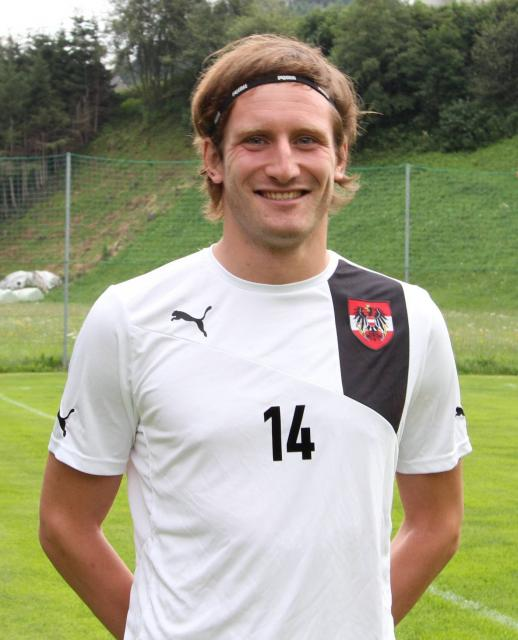
\includegraphics[width=4cm]{images/leitnerBeisp.jpg}
	\caption{Michael Leitner}
\end{figure}
	\textbf{Name:} Micahel Leitner\\
\textbf{Funktion:} Projekt Leiter\\
\textbf{Wohnort:} Oberperfuss\\
\textbf{E-Mail:} mleitner@tsn.at\\
\textbf{Aufgabenbereiche:} \begin{itemize}
	\item Steuerung
	\item Tiem-Rift-Prinzip
	\item Dokumentation
\end{itemize}
\newpage
\subsection{Betreuer}
Seitens der Schule hat sich Herr Claudio Landerer bereiterklärt unser Projekt zu Betreuen. Er brachte uns in seinem Unterricht das Programmieren bei. 
	\begin{figure}[H]
		\centering
		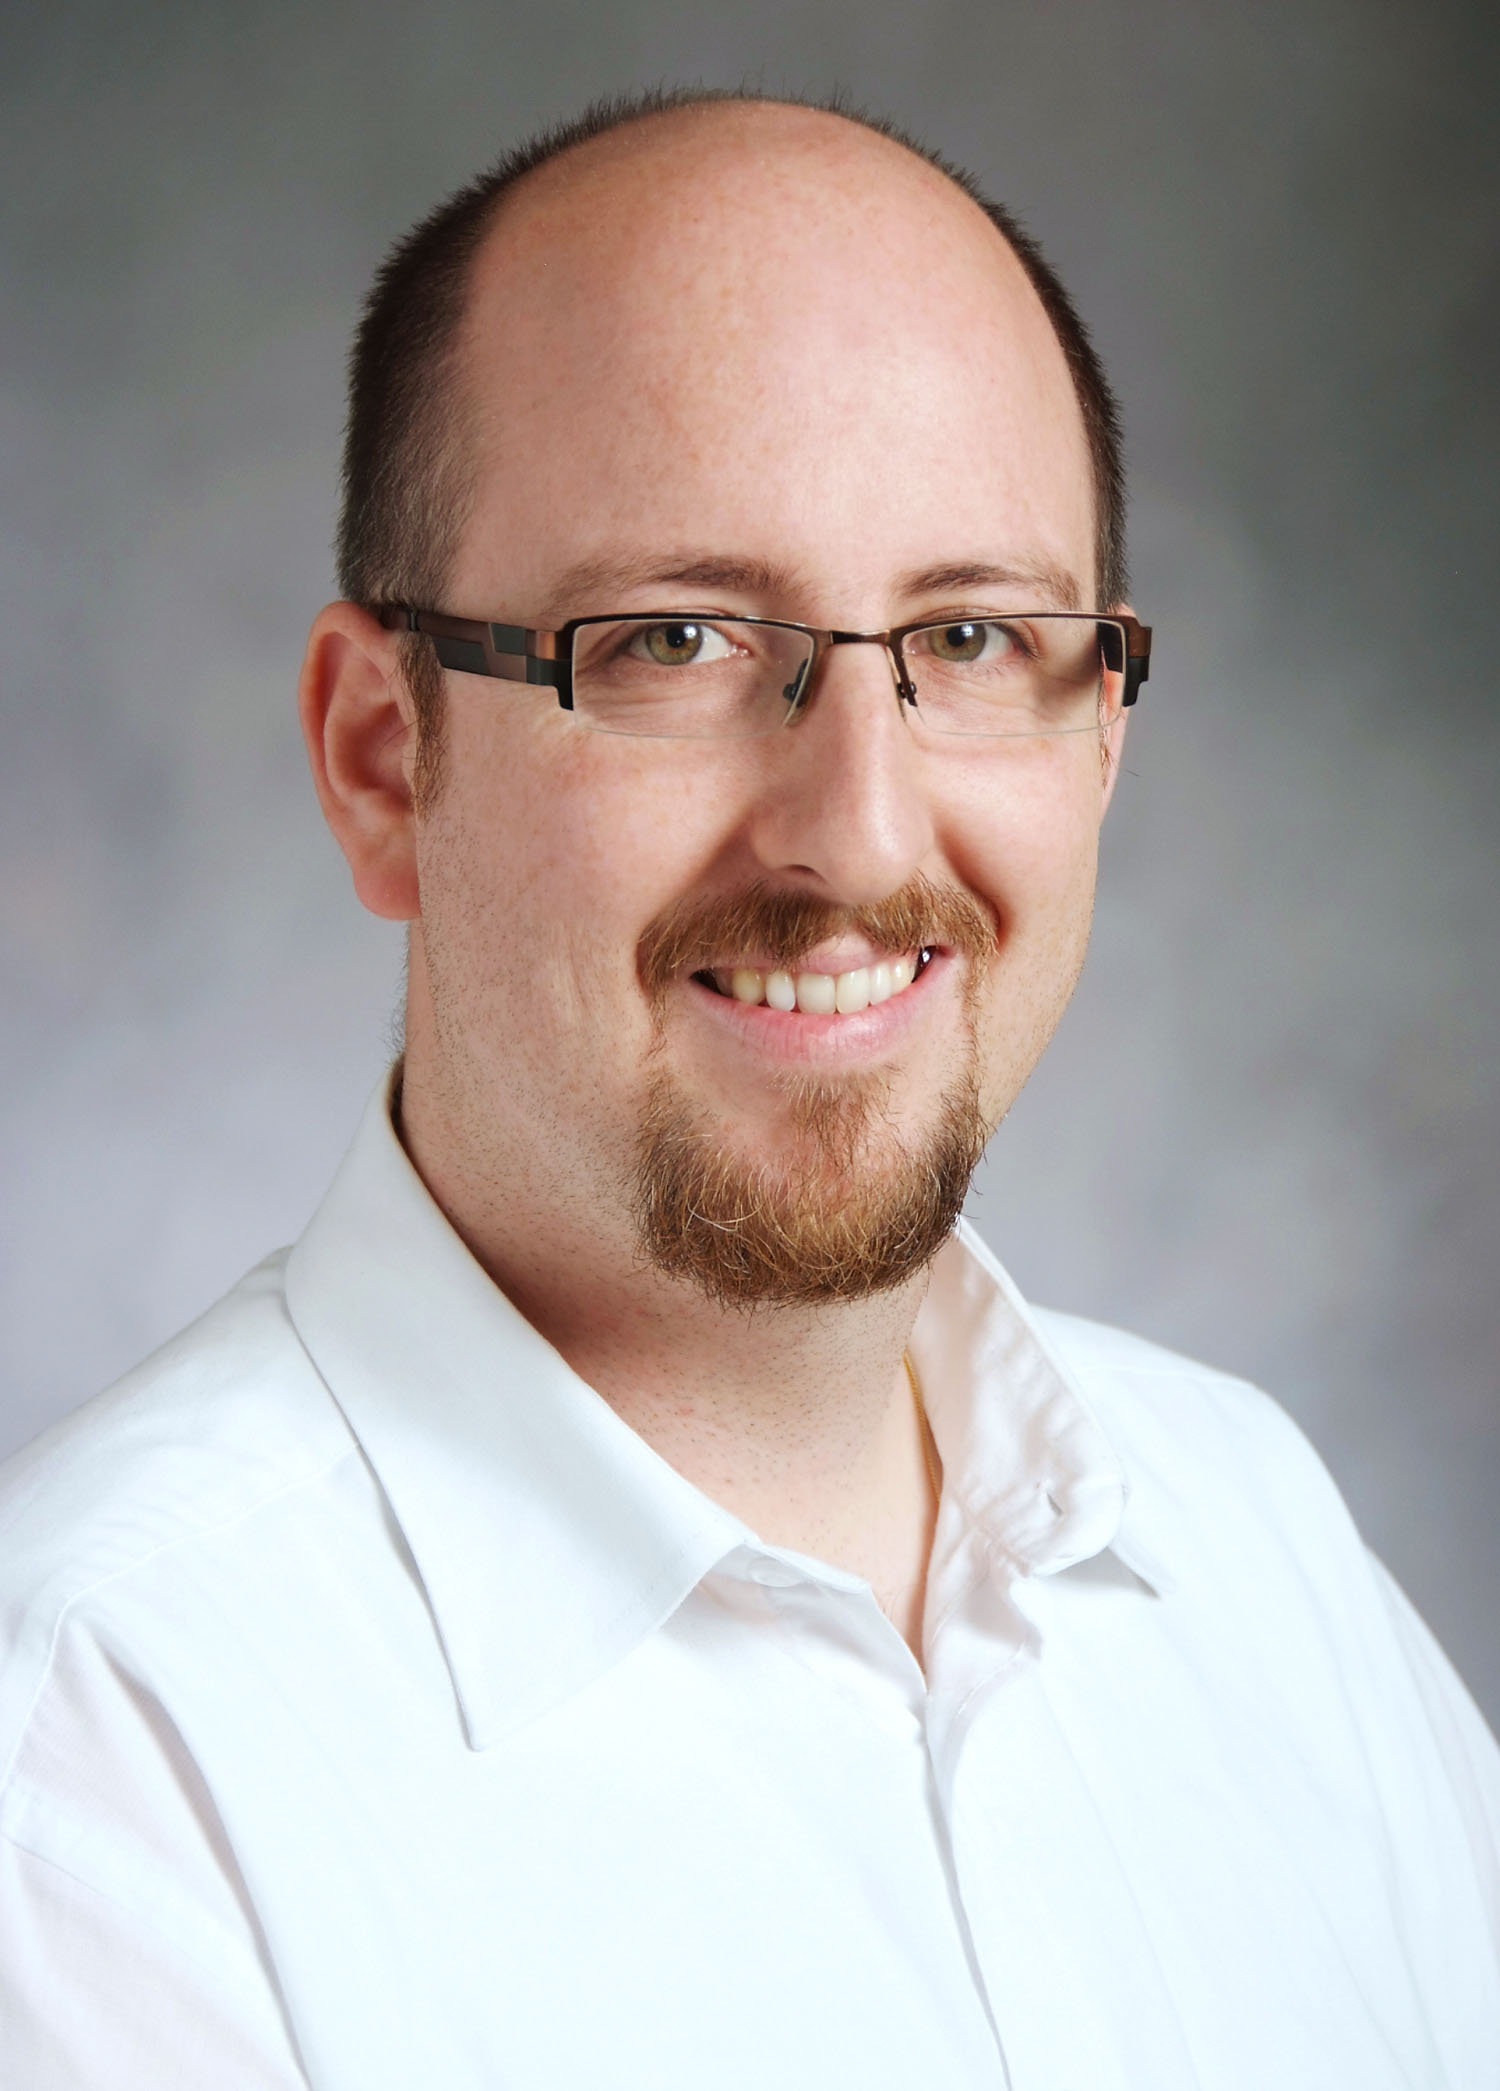
\includegraphics[width=4cm]{images/Landerer_Claudio.jpg}
		\caption{Mag. Claudio Landerer}
	\end{figure}
		
\newpage
\subsection{Partner}
\begin{figure}[H]
	\centering
	
\includegraphics[]{images/ClockstoneLogo.png}
	\caption{ClockStone Softwareentwicklung GmbH}
\end{figure}
Unser Partner während der Diplomarbeit war die Firma ClockStone Softwareentwicklung GmbH. ClockStone ist eine Spielentwicklungsunternehmen mit Sitz in Innsbruck, das im Jahr 2006 gegründet wurde. Einige ihrer Produkte wie zum Beispiel Bridge Constructor sind weltweit bekannt und sehr beliebt. 


\subsection{Ansprechpartner}
Unser Ansprechpartner des Unternehmens war Michael Schiestl. Er unterstütze uns bei Fragen bezüglich der Spielentwicklung und es war äußerst angenehm mit ihm zu arbeiten.

\begin{figure}[H]
	\centering
	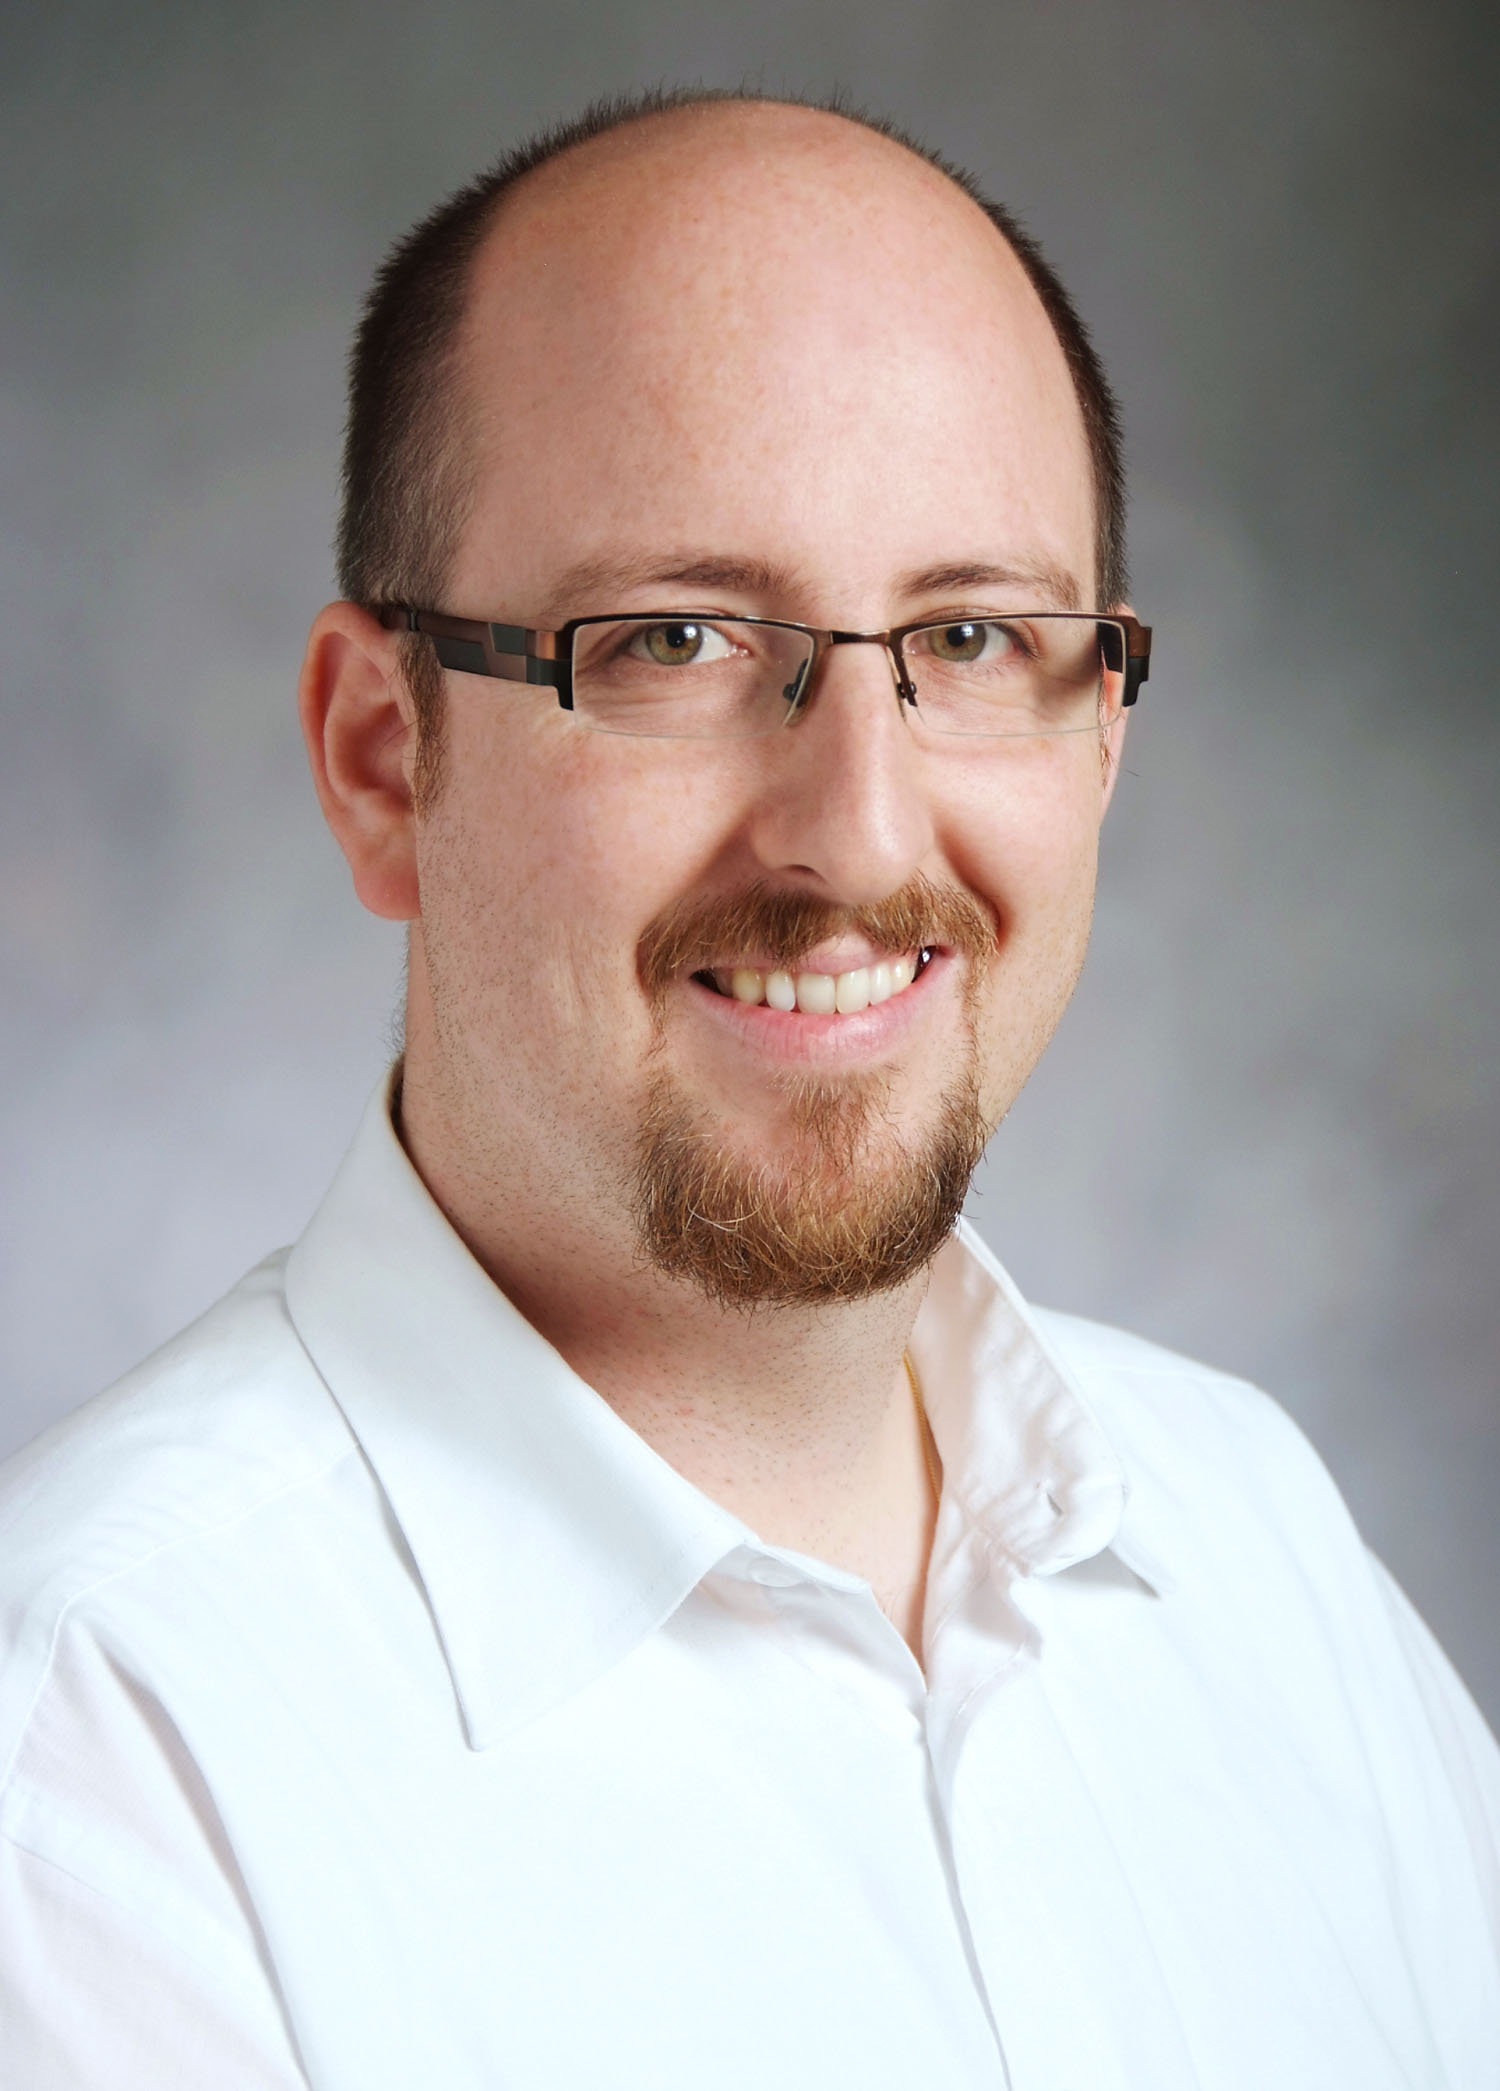
\includegraphics[width=3cm, height=4cm]{images/Landerer_Claudio.jpg}
	\caption{Michael Schiestl}
\end{figure}
\section{Vorerhebungen}
\subsection{Projektzieleplan}
\def \currentAuthor {Michael Leitner} Das Ziel unseres Projekts ist es ein spielbares, unterhaltendes und einfach bedienbares Computer
Spiel zu entwickeln. Die Meilensteine sollen Termingerecht realisiert werden und es soll pünktlich bis
zur Projektabgabe im Juni fertig gestellt werden.
\newpage
\subsection{Projektumfeld}
\def \currentAuthor {Lukas Vogel} %so kann jederzeit der Autor geändert werden -> wird in der Fusszeile angezeigt.
\subsubsection{Stakeholder-Analyse}
Die Ergebnisse der Stakholder-Analyse zu sehen in Tabelle \ref{Stakeholder-Analyse}:
\begin{table}[H]
		
	\renewcommand{\arraystretch}{1.5}
		\begin{tabular}{|p{3cm}|p{6cm}|p{3cm}|p{1.5cm}|p{1.5cm}|}
			\hline
			\textbf{Stakeholder} & \textbf{Beschreibung} & \textbf{Einstellung} & \textbf{Nähe zum Projekt} & \textbf{Einfluss} \\
			\hline
			Projektteam & Das Team ist dem Projekt positiv eingestellt und hofft, sich neues Wissen aneignen zu können. & sehr positiv & 10 & 10\\
			\hline
			Landerer Claudio & Betreuer des Projekts. & neutral & 9 &10\\
			\hline
			ClockStone Softwareentwicklung GmbH.& Projektpartner der Diplomarbeit & positiv & 9 & 10\\
			\hline
			Stefan Walch & Direktor der Schule und Studienkoordinator & neutral& 5 & 10\\
			\hline
			Andere Lehrpersonen & Die anderen Lehrpersonen des IT-Kollegs sind während allen Präsentationen anwesend und können die Notengebung beeinflussen & neutral& 2 & 4\\
			\hline
			Mitschüler & Manche Klassenmitglieder spielen gerne am Computer in der Freizeit	& neutral bis positiv & 1 & 1\\
			\hline
		\end{tabular}
\caption{Stakeholder-Analyse}
\label{Stakeholder-Analyse}
	\end{table}
Die Einschätzung der Einstellung, der verschiedenen Stakeholder zum Projekt, in Tabelle \ref{Stakeholder-Analyse} geht von sehr negativ über neutral bis zu sehr positiv. Der Einfluss auf die Diplomarbeit wiederum wird mit einer Skala von 1-10 beschrieben, wobei 1 keinen bzw. sehr wenig Einfluss repräsentiert und 10 sehr starken. Auch die Nähe zum Projekt wird von 1-10 skaliert, 1 repräsentiert weit entfernt vom Projekt und 10 sehr nah.
\subsubsection{Stakeholder-Diagramm}
\begin{figure}[H]
	\centering
	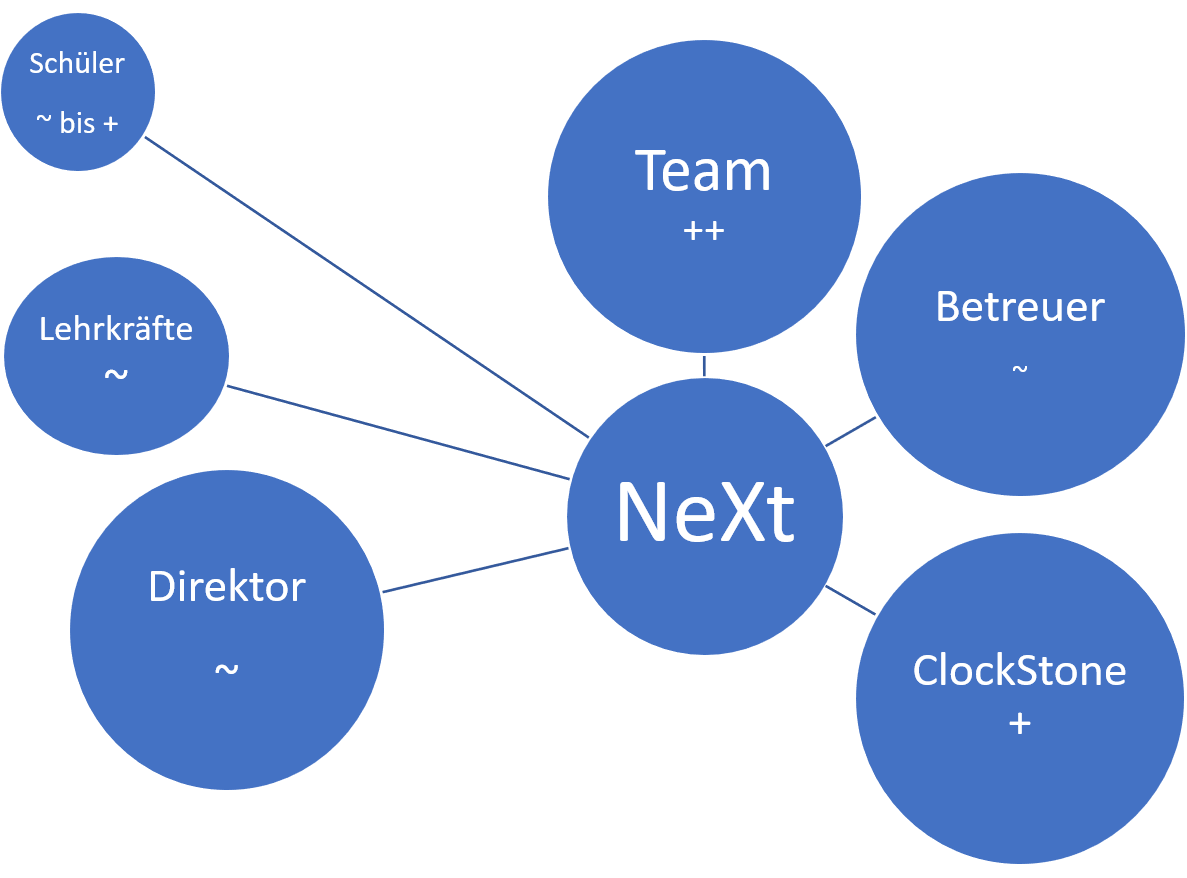
\includegraphics[width=16cm,height=8cm]{images/Projektumfeldanalyse.png}
	\captionbelow{Stakeholder-Diagramm}
	\label{Stakeholder-Diagramm}
\end{figure}
	In diesem Diagramm, Abbildung \ref{Stakeholder-Diagramm} ist das Ergebnis der Tabelle \ref{Stakeholder-Analyse} graphisch dargestellt. Die Größe der Kreise Zeigt den Einfluss, die Länge der Linien zwischen Stakeholder und NeXt die Nähe und die Zeichen (++ --> sehr positiv, ~ --> neutral, -- --> sehr negativ) unter dem Namen des Stakeholders dessen Nähe zum Projekt. 

\subsection{Risikoanalyse}
\begin{figure}[H]
	\centering
	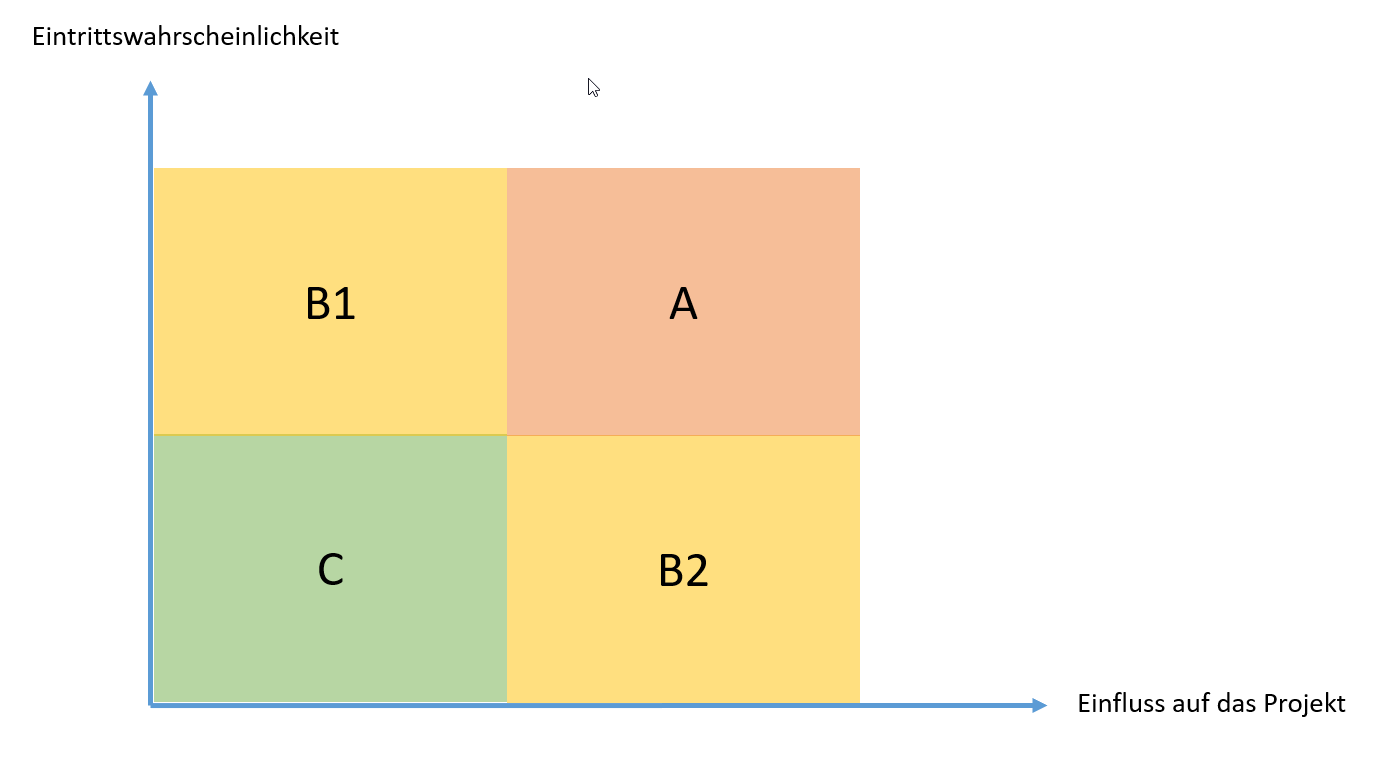
\includegraphics[width=16cm,height=8cm]{images/Risiko-Matrix.png}
	\caption{Matrix zur qualitativen Einordnung von Risiken}
	\label{MatrixRisiken}
\end{figure}
 Die Matrix (Abb. \ref{MatrixRisiken}) wurde in vier Kategorien eingeteilt. Die Risiken werden dann zur jeweils passende Kategorie ein zugeordnet um diese dann besser einschätzen zu können.\cite[S. 141 -142]{SystemplanungundProjektmanagement-Lehrbuch}

Folgende Risiken sind aus der Projektumfeld-Analyse hervorgegangen und werden in Tabelle \ref{Risiko} beschrieben, bewertet und Maßnahmen gesetzt.

	\begin{table}[H]
			\centering
		\renewcommand{\arraystretch}{1.5}
		\begin{tabular}{|p{3cm}|p{5cm}|p{2cm}|p{5cm}|}
			\hline
			\textbf{Risiko} & \textbf{Beschreibung} & \textbf{Bewertung} & \textbf{Maßnahme} \\
			\hline
			Motivation des Teams & Die Motivation des Teams ist sehr wichtig. Wenn die sie sinkt, verringert sich auch die Arbeitsmoral, dies führt zu weniger Produktivität, was wiederum zum totalen Stillstand der Diplomarbeit führen kann. & A & Um die Wahrscheinlichkeit zu reduzieren sind am Anfang möglichst schnell Erfolgserlebnisse zu erzielen, dies steigert die Motivation sehr gut. Zusätzlich hilft es bei Problemen nicht Stunden lang am Problem zu sitzen, sondern entweder an etwas Anderem zu arbeiten oder jemanden um Hilfe zu bitte.\\
			\hline
			Zufriedenheit des Betreuers & Herr Landerer ist der Betreuer des Projekts und wenn er nicht mit unseren Leistungen zufrieden ist kann er das Projekt stoppen. & B2 & \begin{itemize}
				\item laufende Berichterstattung
				\item laufender Fortschritt im Projekt
				\item bei Problemen oder Verzögerungen mit ihm reden
			\end{itemize}\\
		\hline
		Zufriedenheit des Partners & Die Firma ClockStone Softwareentwicklung GmbH soll wie der Betreuer mit dem Fortschritt und dem Projekt an sich zufrieden sein. Da auch sie im extrem Fall das Projekt zum Stopp zwingen könne. & B2 & Auch hier kann eine laufende Berichterstattung und vor allem Meetings mit dem Partner helfen. Des weiteren ist zu beachten, dass auch ihr Unternehmen Spiele entwickelt, dadurch können sie bei Problemen kontaktiert werden, was zu einer schnelleren Lösungsfindung führen kann und somit auch ihren Wünschen entspricht.\\
		 \hline
		\end{tabular}
	\end{table}
\newpage
\begin{table}[H]
	\centering	
		\renewcommand{\arraystretch}{1.5}
	\begin{tabular}{|p{3cm}|p{5cm}|p{2cm}|p{5cm}|}
		\hline
		Zufriedenheit des Direktors & Herr Walch ist auch für die Abnahme des Projekts zuständig. Wenn das Projekt seinen Anforderungen nicht entspricht kann er das Projekt abbrechen. Darüber hinaus  ist er bei den Präsentationen der Diplomarbeit anwesend, dort werden von den allen Lehrern auch Fragen zum Projekt gestellt. Wenn diese nicht eine fachlich kompetente Antwort bekommen, kann das einen negativen Einfluss auf das Projekt haben. & B2 & Um dieses Risiko zu abzuschwächen ist es besonders wichtig auf die Fragen und Anmerkungen von Herrn Walch einzugehen. Deswegen ist es essentiell sich gut auf die Präsentationen vor zu bereiten.\\
		\hline
		Zufriedenheit der anderen Lehrpersonen & Wie Herr Walch, sitzen auch andere Lehrpersonen während der Personen dabei und können Fragen zum Projekt stellen. & C & Dieses Risiko kann mittels guter Vorbereitung bei den Präsentationen verringert werden. \\
		\hline
	\end{tabular}
		\caption{Risiko-Bewertung-Maßnahmen}
\label{Risiko}
\end{table}
\section{Pflichtenheft}
\subsection{Zielbestimmung}
Das Spiel „NeXt“ soll nach dem „Time-Rifts“-Prinzip agieren.
Das 2-Dimensionale Spiel wird gemeistert durch:
\begin{itemize}
	\item koordinierte Zusammenarbeit aller Figuren
	\item Zeitmanagement
	\item Jump-and-Run Elemente
	\item Lösen von Puzzle-Elementen
\end{itemize}
\begin{figure}[H]
	\centering
	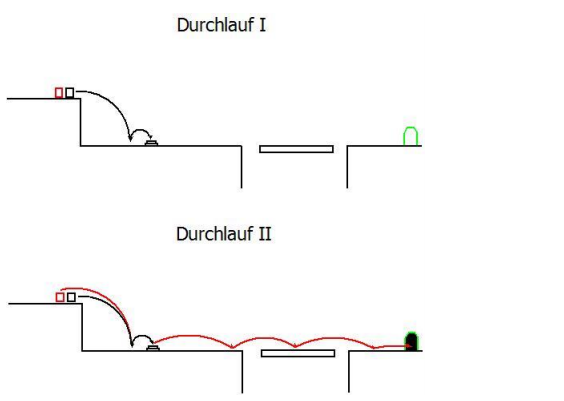
\includegraphics[width=10cm]{images/TimeRift.png}
\end{figure}
Time-Rifts (Erklärung): Jeder Durchlauf hat ein Zeitlimit, dass Ziel sollte es sein Durch die
verschlossene Tür (grün) zu gehen.
\begin{itemize}
	\item Durchlauf I:
	Der/die Spieler/in bewegt Figur 1(schwarzes Rechteck) auf eine Bodenplatte.
	-> Tür öffnet sich. (bleibt offen solange die Bodenplatte betätigt ist)
	\item Durchlauf II:
	Figur 1 macht das selbe wieder (in Echtzeit) und der/die Spieler/in bewegt Figur 2 (rotes
	Rechteck) durch die Tür
\end{itemize}
Jedoch ist dieses Prinzip nicht auf nur 2 Durchgänge beschränkt.
\subsection{Produkteinsatz und Umgebung}
Die Zielgruppe dieses Spieles, ist jeder der sich einer Herausforderung stellen möchte. Durch das TimeRift-Prinzip wird eine großer Herausforderung geboten.Spielbar wird dieses Spiel auf jedem Windows-Computer sein. Da auf gute Grafik verzichtet worden ist, muss der Computer auch nicht leistungsstark sein, um das Spiel ausführen zu können 
\subsection{Funktionalitäten}
\begin{itemize}
	\item MUSS-Anforderungen
	\begin{itemize}
		\item Funktional:
		\begin{itemize}
			\item TimeRift-Prinzip-Implementiert
			\item Ein paar Level implementiert
		\end{itemize}
		\item Nicht-funktional
		\begin{itemize}
			\item Das Spiel soll einfach gesteuert werden
			\item Das Spiel soll Einschränkungen Spielbar sein.
		\end{itemize}
	\end{itemize}
	\item KANN-Anforderungen
	\begin{itemize}
		\item Funktional
		\begin{itemize}
			\item Ein Komplettes Level-Pack enthalten
			\item Erweiterte Steuerungsmöglichkeiten 
		\end{itemize}
		\item Nicht-funktional
		\begin{itemize}
			\item Das Spiel kann mit Musik unterlegt sein
		\end{itemize}
	\end{itemize}
\end{itemize}
\section{Planung}
\subsection{Projektstruktrplan}
\begin{figure}[H]
	\centering
	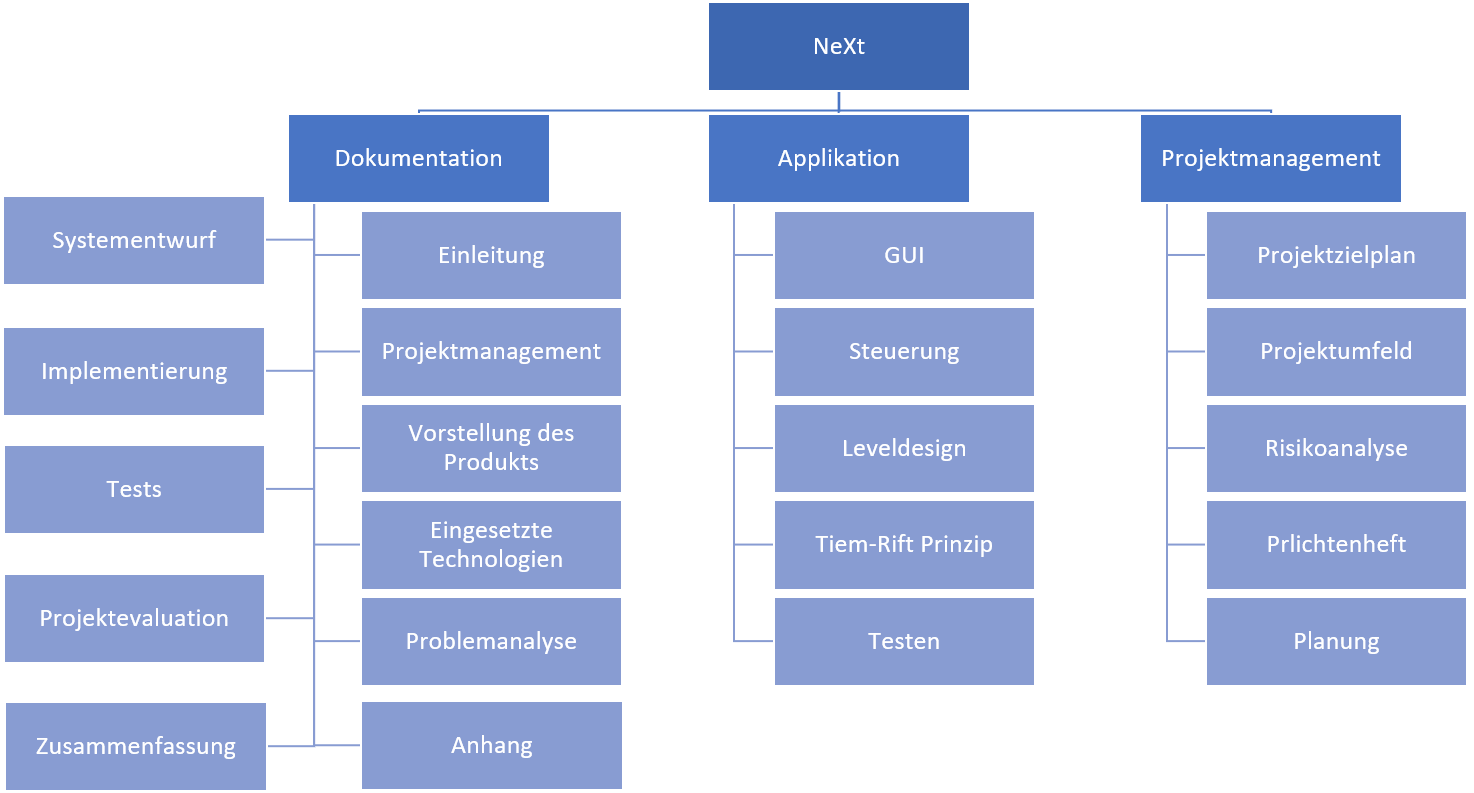
\includegraphics[width=16cm,height=8cm]{images/Projektstrukturplan.png}
	\captionbelow{Projektstrukturplan}
	\label{Projektstrukturplan}
\end{figure}

Der Projektstrukturplan, zu sehen in Abbildung \ref{Projektstrukturplan}, soll den gesamten Umfang des Projekts strukturiert und gut lesbar darstellen.

\subsection{Meilensteine}\begin{itemize}
	\item 10.10.2017 Abschluss Anforderungsdefinition, Vorbereitung der Entwicklungsumgebung	
	\item 28.11.2017 Erster spielbarer Prototyp (Basissteuerung, Physik, Sound, Grafik, Test-Level)	
	\item 09.01.2018 Spielbarer Prototyp nach dem Timerift-Prinzip	
	\item 06.02.2018 Erste spielbare Levels	
	\item 20.03.2018 Vollständige Fertigstellung des Spiels mit einigen Levels, Beginn der Beta-Testing-Phase	
	\item 06.04.2018 Abschluss Beta-Testing	
	\item 30.04.2018 Verbesserung des Prototyps auf Basis der Rückmeldungen (Beta-Test)
	\item 15.06.2018 Fertigstellung der Dokumentation, Übergabe an den Auftraggeber
\end{itemize}
\subsection{Gant-Chart}

\subsection{Pläne zur Evaluierung}
\subsection{Ergänzungen und zu klärende Punkte}
\chapter{Vorstellung des Produktes}
\section{Produktbeschreibung}
Das Computerspiel NeXt ist in den Genres Jump and Run und Puzzle angesiedelt. Hauptaugenmerk dieses Spiels ist das sogenannte „Time-Rift“ Prinzip. Bei diesem Prinzip geht es darum, dass der Spieler jedes Level mehrmals in einzelnen Durchläufen spielen wird. Der Clue an der Sache ist jedoch, dass die zuvor gespielten Charaktere sich genauso bewegen wie sie in den vorigen Durchläufen gesteuert wurden. Das heißt: Hat der Spieler mit dem ersten Charakter einen Schalter betätigt, der eine Tür öffnet, dann wiederholt der Charakter diesen Vorgang, nur diesmal von selbst. Währenddessen kann der Spieler mit dem zweiten Charakter zu der zuvor genannten Tür gehen, welche sich öffnet, da der erste Charakter wieder den Schalter betätigt und somit wird das Level beendet. Durch dieses besondere Spielprinzip können vollkommen neue Puzzele-Elemente in das Produkt eingebaut werden, dies soll den Reiz des Spiels ausmachen.  Damit das Spiel aber nicht zu leicht wird, wird noch ein Zeitfaktor eingebaut, welcher den Spieler unter Druck setzten soll. Schafft der Spieler nicht den Schalter in der geforderten Zeit zu betätigen, so wird er mit dem zweiten Charakter nicht durch die Tür kommen und kann deshalb nicht das Level beenden. Durch ein abwechslungsreiches Level Design und das oben beschriebene Spielprinzip soll ein interessantes Spiel entwickelt werden das auch einen großen Wiederspielfaktor als Ziel hat. Die Benutzeroberfläche so wie das Spielgefühl sollen intuitiv sein und für alle User keine große Umstellung zu anderen Spielen sein. Die genauen Mechaniken sowie die Funktionsweise des Spiels wurden in der Dokumentation erläutert.  
\chapter{Eingesetzte Technologien}
\section{Engine}

\subsection{Spiel-Engine}
Eine Spiel-Engine ist eine Art Framework, welches spezielle für Computerspiele entwickelt wurde. Die Engine ist zuständig für den Spielverlauf aber auch für die visuelle Darstellung des Spielablaufs. Viele Spiel-Engines liefern eine Entwicklungsumgebung mit, diese liefert die Werkzeuge für die Entwicklung der jeweiligen Applikation mit. \cite{Spiel-Engine}

\subsection{Unity-Engine}
Auf anraten unseres Projektpartners verwendeten wir die Unity-Enigne, da das Unternehmen selbst damit arbeitet. Die Engine liefert eine Entwicklungsumgebung mit. Wir empfanden die Arbeit mit der Unity als angenehm. Zusätzlich ist es eine sehr weit verbreitete Spiel-Engine zu der es auch äußerst hilfreiches Lehrmaterial gibt. Unity selbst bietet auch eine Vielzahl an Lernvideos an.

Das Unternehmen Unity Technologies hat seine Hauptsitz in San Francisco und wurde 2004 gegründet. Die Zielplattformen für Unity sind PCs, Spielkonsolen, mobile Geräte sowie Webbrowser. \cite{Unity-Engine}

\subsubsection{Technische Eigenschaften}
Nachstehend werden die wichtigsten Technische Eigenschaften der Unity-Engine erklärt. 

\textbf{Grafik}\\
Unity ist auf dem neusten Stand der Technik und unterstützt die verschiedensten Techniken die derzeit in der Spielentwicklung benötigt werden. Außerdem können die eingebauten Beleuchtungseffekte selbst bearbeitet werden. Dies erweitert die Möglichkeiten der Engine nochmals signifikant.

\textbf{Animation}\\
Objekte des Spiels könne über Skripte und andere Vorgehensweisen wie zum Beispiel physikalische Kräfte bewegt werden. Dieser Mechanismus war für unser Projekt sehr wichtig da der Spieler die Charaktere selbst in Echtzeit steuert. 

\textbf{Programmierung}\\
Unity unterstützt drei verschiedene Programmiersprachen:
\begin{itemize}
	\item C\#
	\item UnityScript (vergleichbar mit JavaScript)
	\item Boo
\end{itemize}
Diese sind notwendig um Skripte zu erstellen, welche die von Unity eingebauten Mechanismen erweitern. Da wir im Unterricht bereits mit C\# Erfahrungen sammeln konnten, haben wir diese verwendet.

\textbf{Werkzeuge}\\
Die Engine ist mittels Werkzeugen erweiterbar, diese sind zu einem Teil kostenlos Verfügbar und als einfache Plug-ins zu integrieren. Bei unserem Projekt konnten wir dadurch ohne Kosten einfache Grafiken und nützliche Tools einsetzen.\\
\cite{Unity-Engine}

\section{Entwicklungsumgebung}
\subsection{Unity-Editor}
Als Entwicklungsumgebung wählten wir Unity-Editor da sie vom selben Unternehmen entwickelt wurde und somit speziell für die Unity-Engine gemacht wurde. Sie wurde basierend auf gängigen 3D-Animationsprogrammen designet. Sie ist sehr einfach zu bedienen und ermöglicht das importieren von Werkzeugen mittels eines einfachen Mausklicks. In dieser Entwicklungsumgebung können alle für die Spielentwicklung wichtigen Arbeiten verrichtet werden. Für das Programmieren der Scripte verwendeten jedoch wir Visual Studio. \cite{Unity-Engine}

\subsection{Visual Studio}
Wir verwendeten für die Programmierung von Scripten Visual Studio Community 2017, welche für Studenten kostenlos ist und wir im Unterricht zum entwickeln von Apllikatione mit C\#  verwendeten. 

\section{C\#}
Im Unterricht hatten wir unseren ersten Kontakt mit der Programmiersprache C\#. Bei diesem Projekt konnten wir unser erlerntes Wissen nutzen, da wir es für die Scripte in Unity verwendeten. 

\section{Dokumentation}
Für die Dokumentation der Diplomarbeit verwendeten wir auf anraten von unserem Betreuer LaTeX in Kombination mit der Applikation TeXstudio.
LaTeX vereinfacht die Benutzung von TeX einem Textsatzsystem mittels Makros. TeXstudio ist eine Entwicklungsumgebung die für LaTeX entwickelt wurde. \cite{Latex}
\chapter{Problemanalyse}
\section{USE-Case-Analyse}
In diesem Projekt wurde eine USE-Case-Analyse vollzogen. Als Benutzer gibt es nur den Anwender der Applikation, dessen Ziel es sein wird das Computerspiel zu spielen oder es zu beenden. Die USE-Case-Analyse und dessen Ergebnis wird als Diagramm in Abbildung \ref{USE-Case-Diagramm} dargestellt.
\begin{figure}[H]
	\centering
	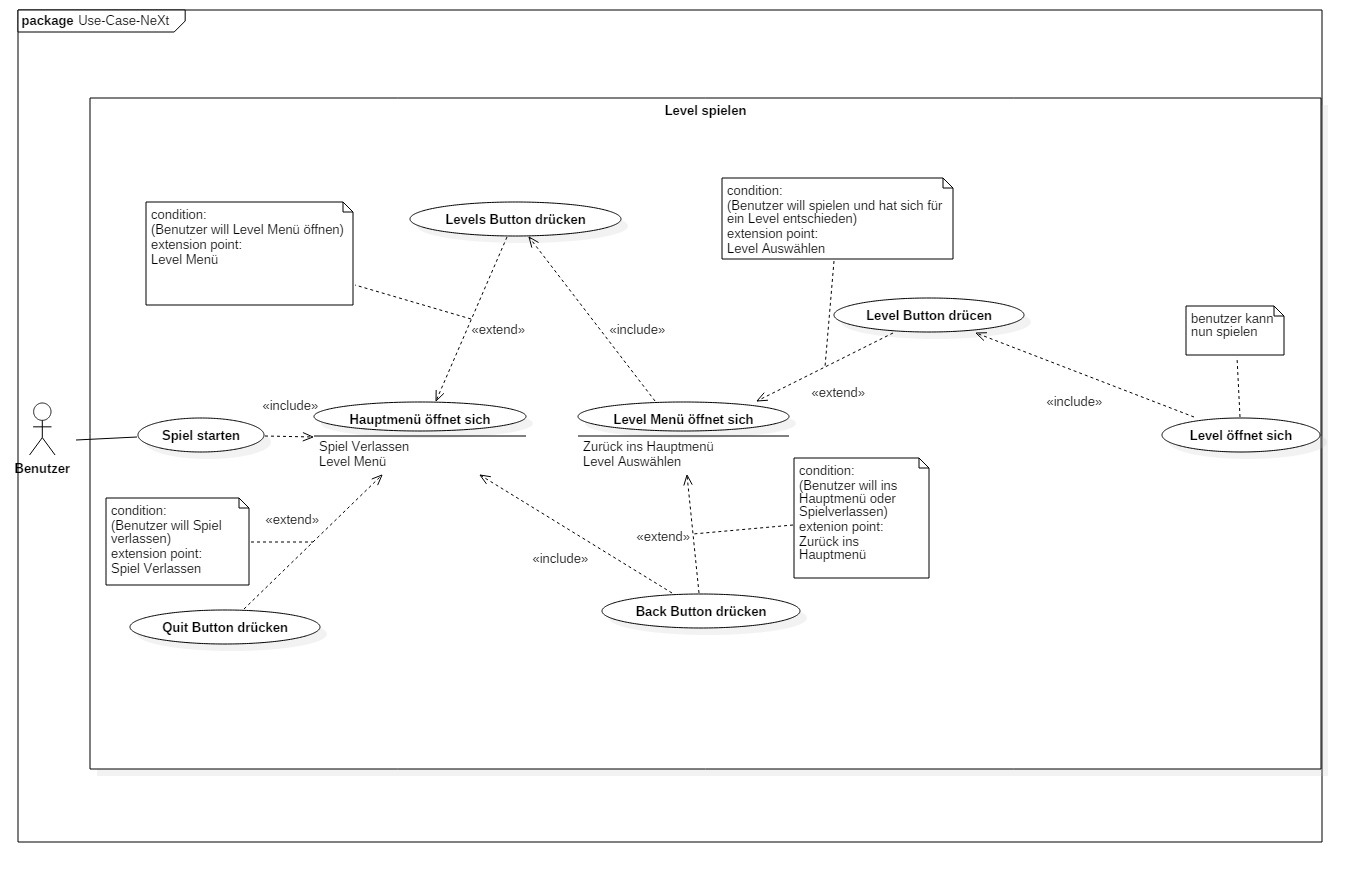
\includegraphics[width=17.5cm,height=10cm]{images/UseCaseDiagram.jpg}
	\caption{USE-Case-Diagramm}
	\label{USE-Case-Diagramm}
\end{figure}
\section{Domain-Class-Modelling}
\begin{itemize}
	\item "Dinge" (Rollen, Einheiten, Geräte, Events etc.) identifizieren, um die es im Projekt geht
	\item ER-Modellierung oder Klassendiagramme
	\item Zustandsdiagramme (zur Darstellung des Lebenszyklus von Domain-Klassen darstellen)
\end{itemize}

\section{User-Interface-Design}
Im folgenden Teil der Dokumentation sind verschiedene Wireframes der Benutzeroberfläche des Programms zu sehen.
\begin{figure}[H]
	\centering
	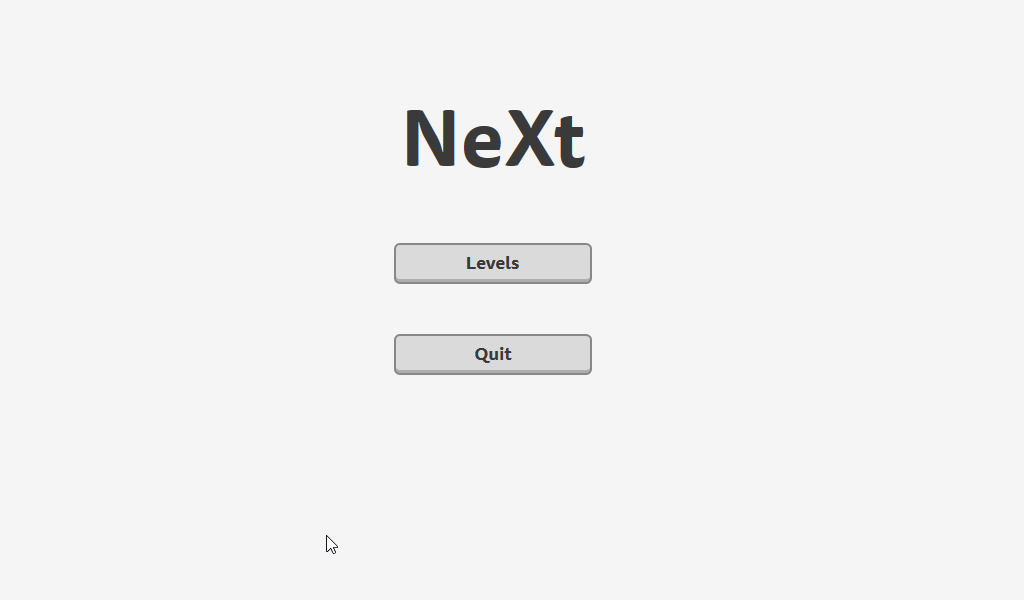
\includegraphics[width=16cm, height=9cm]{images/WireframeMainmenu.png}
	\caption{Wireframe-Hauptmenü}
	\label{WireframeMainmenu}
\end{figure}
In Abbildung \ref{WireframeMainmenu} ist der erste Entwurf für das Hauptmenü des Spiels zu sehen. Diese Ansicht ist die Erste die der Benutzer sehen soll wenn er das Computerspiel startet. Das Menü ist sehr einfach gehalten. Es gibt ein Textfeld welches "NeXt" anzeigt und darunter zwei Buttons. Der obere Button soll  den Spieler in das Menü der Levels leiten, siehe Abbildung \ref{WireframeLevelsmenu}. Der untere Button soll  die Applikation schließen.
\begin{figure}[H]
	\centering
	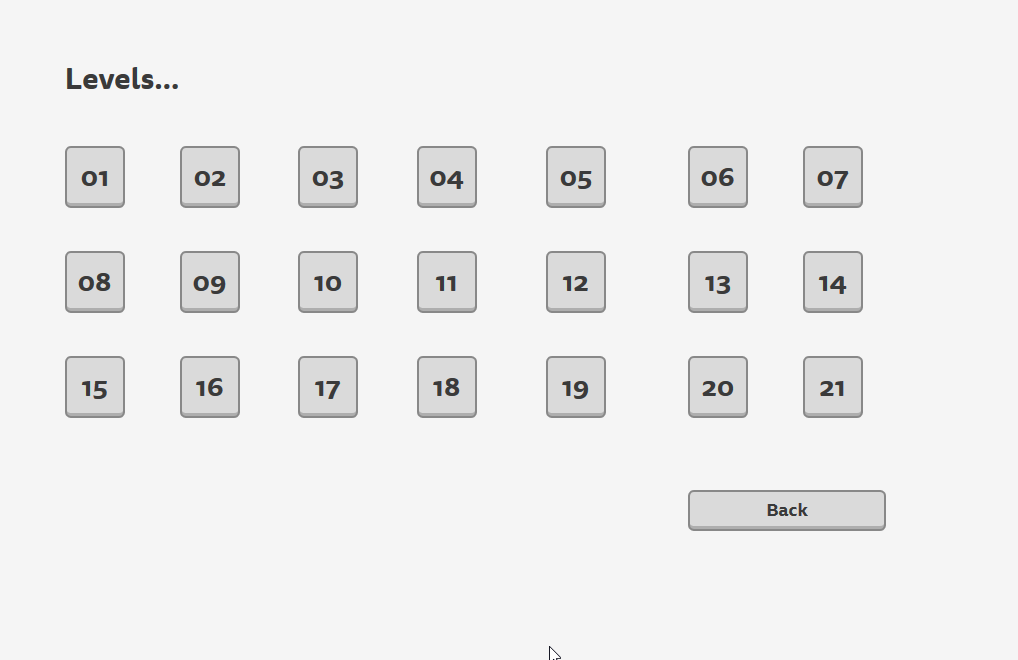
\includegraphics[width=16cm, height=9cm]{images/WireframeLevelsmenu.png}
	\caption{Wireframe-Levelmenü}
	\label{WireframeLevelsmenu}
\end{figure}
Das nächste Wireframe in Abbildung \ref{WireframeLevelsmenu} zeigt eine Übersicht aller Spielbaren Levels welche als Nummerierte Buttons dargestellt werden. Wenn der Benutzer einen Level-Button betätigt soll  sofort das gewählte Level starten. Der Button rechts unten mit der Beschriftung "Back" soll den Spieler wieder zurück in das Hauptmenü führen. 
\begin{figure}[H]
	\centering
	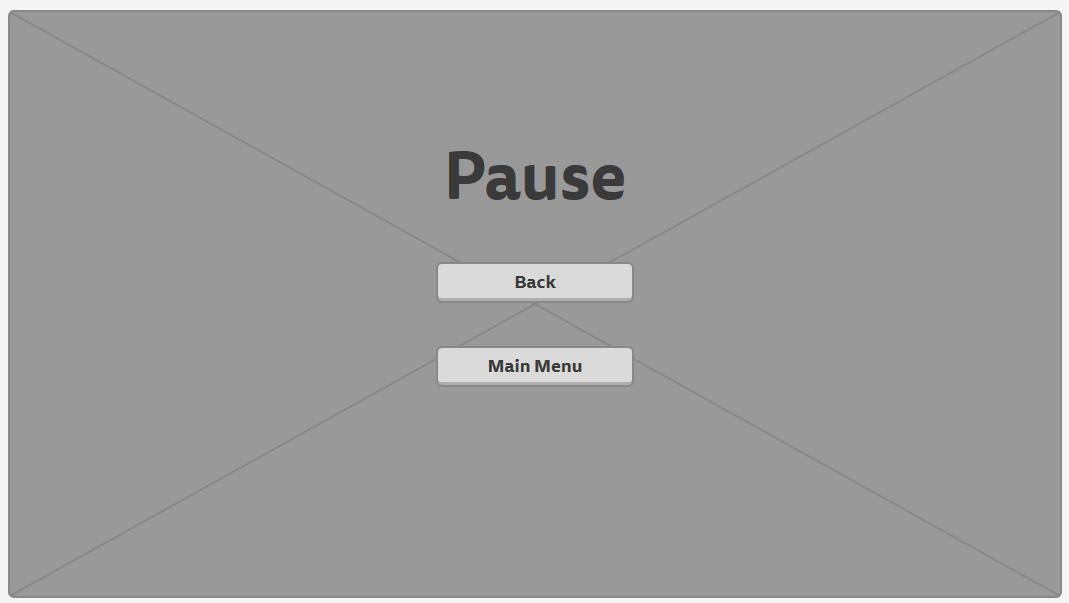
\includegraphics[width=16cm, height=9cm]{images/WireframePausemenu.png}
	\caption{Wireframe-Pausemenü}
	\label{WireframePausemenu}
\end{figure}
Sobald der Benutzer sich in einem Level befindet soll er die Möglichkeit habben, mittels Escape-Taste das Spiel stoppen und in das Pausemenü wechseln. Das Wireframe dazu ist in Abbildung \ref{WireframePausemenu} zu sehen. Die graue Fläche soll dabei das Level darstellen welches im Hintergrund immer noch zu sehen sein soll. Zusätzlich sind noch zwei Buttons zu sehen der erste Button mit dem Text "Back" soll das Menü wieder schließen und das Spiel weiter laufen lassen. Der Zweite welcher mit der Beschriftung "Main Menu" versehen ist soll denn Benutzer wieder in die Ansicht des Hauptmenüs, Abbildung \ref{WireframeMainmenu} bringen. 
\chapter{Systementwurf}

\section{Architektur}

\subsection{Design der Komponenten}
In der Unity3D Entwicklungsumgebung werden keine Klassischen Architekturmuster verwendet. Wenn ein bestimmtes Objekt ein Skript benötigt, wird ihm dieses Skript angehängt. Jedoch wurden für das TimeRift-Prinzip mehrere Klassen verwendet.


UML!!!

\chapter{Implementierung}
\section{GUI}
\section{Leveldesign}

\begin{itemize}
	\item GUI-Implementierung
	\item Controllerlogik
	\item Geschäftslogik
	\item Datenbankzugriffe
\end{itemize}

Detaillierte Beschreibung der Teststrategie (Testdriven Development):

\begin{itemize}
	\item UNIT-Tests (Funktional)
	\item Integrationstests
\end{itemize}

Zu Codesequenzen:
\begin{itemize}	\item kurze Codesequenzen direkt im Text (mit Zeilnnummern auf die man in der Beschreibung verweisen kann)
	\item lange Codesequenzen in den Anhang (mit Zeilennummer) und darauf verweisen 
\end{itemize}

\section{Unity-Klassenstruktur}
\subsection{MonoBehaviour}	
Die Klasse „MonoBehaviour“ ist eine Standardklasse, die von der Unity3D-Engine bereitgestellt wird. Jedes Skript, welches in Unity verwendet wird, muss von dieser Klasse erben (Ähnlich wie in Java die „Object-Klasse“ von jeder Klasse gerbt wird). MonoBehaviour gibt folgende Methoden zur Verfügung:
\begin{itemize}
	\item Start()
	\item Update()
	\item FixedUpdate()
	\item LateUpdate()
	\item OnGUI()
	\item OnDisable()
	\item OnEnable()
\end{itemize}
Verwendet werden in diesem Projekt aber nur die Start, Update, FixedUpdate und LateUpdate Methoden.
\subsection{Start-Methode}
Die Start-Methode wird nur einmal in der Skriptlaufzeit aufgerufen und zwar bei der Initialisierung des Skriptes.
\subsection{Update-Methode}
Die Update-Methode wird bei jedem Frame aufgerufen. Sie wird meistens für Berechnungen, die in jedem Frame durchgeführt werden müssen, verwendet. Nachteil hier ist aber, wenn das Spiel eine schlechte Framezahl hat werden die Berechnungen auch weniger oft durchgeführt.
\subsection{FixedUpdate-Methode}
Die FixedUpdate-Methode wird bei jedem fixierten Framerate Frame aufgerufen. Diese Methode soll verwendet werden für Bewegungen eines Charakters (Spielbar und nicht Spielbar). Dies hat den Grund, dass selbst bei schlechter Framerate, die Berechnungen der Bewegung konstant bleiben.
\subsection{LateUpdate-Methode}
Die LateUpdate-Methode wird nach allen anderen Update-Methoden aufgerufen. Sie wird hauptsächlich für Funktionen verwendet die nach all den Update-Methoden aufgerufen werden soll z.b.: Für die Kameraführung, da sich Objekte in der Update-Methode bewegt haben können.
\section{Spieler}
Der Spieler steuert mehrere spielbare Charaktere im laufe  eines Levels. Damit aber auch die Eingaben des Spieler verwertet werden, werden Skripte benötigt, die diese eingaben auswerten und verwerten. Diese Aufgabe wird von dem PlayerController Skript übernommen. 
\subsection{PlayerController}
Damit der Charakter überhaupt Bewegungen ausführen kann, wurde ihm ein Rigidbody2D-Container angehängt.
\begin{figure}[htbp] 
	\centering
	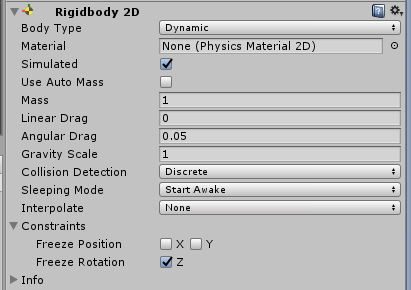
\includegraphics[width=0.7\textwidth]{images/Ridigbody2D.png}
	\caption{Aufbau des Ridigbody2D Containers}
\end{figure}
In diesem Container können verschiedene Eigenschaften, die sich auf den Charakter auswirken, verändert werden. Unter anderem die "Mass" Eigenschaft, welche für das Gewicht des Charakters zuständig ist.

\begin{lstlisting}[language={[Sharp]C}]
void FixedUpdate ()
{
grounded = Physics2D.OverlapCircle(groundCheck.position, groundRadius, whatIsGround);

float move = Input.GetAxis("Horizontal");
Rigidbody2D rb = GetComponent<Rigidbody2D>();
rb.velocity = new Vector2(move * maxSpeed, GetComponent<Rigidbody2D>().velocity.y);

if (move > 0 && !faceingRight)
Flip();
else if (move < 0 && faceingRight)
Flip();
}
\end{lstlisting}

Wie schon bei Punkt 7.1.4 besprochen, wurde hier die FixedUpdate-Methode verwendet, da eine Bewegung unabhängig von der Framezahl berechnet werden soll. Am Anfang der Methode wird überprüft ob sich der Charakter auf dem Boden befinden. Hierfür wird der Funktion "OverlapCircle" die Parameter für den "groundCheck", "groundRadius" und "whatIsGround" mitgegeben
\begin{itemize}
	\item Das "groundCheck" Objekt ist ein unsichtbares Objekt, das dem Charakter angehängt worden und ist dafür zuständig, das sich der Boden und der "groundCheck" überschneiden.
	\item "groundRadius" legt den Radius fest in dem sich der Boden und "groundCheck" überschneiden müssen, damit die Funktion einen boolschen "true" Wert zurückgibt.
	\item "whatisGround" hat die Funktion, der Funktion zu sagen, welche Objekte überhaupt als Boden zählen.
\end{itemize}
Diese Zeile dient dazu, das der Charakter springen kann.

Die Zeilen 6-13  sind für die Bewegung zuständig. In Zeile 6 wird der Input des Spielers eingelesen, wobei nur der Input für die Horizontale Bewegung wahrgenommen wird.
In der Zeile 8 wird dann die Bewegung mittels einer Vektor Berechnung ausgeführt.
Die Zeilen 10-13 sind für die Änderung der Richtung verantwortlich, wobei beide aber nur die Flip-Methode aufrufen. In der Flip-Methode wird letztendlich nur der Charakter gedreht, damit er sich in eine andere Richtung bewegen kann.
Für das Springen des Charakters ist ebenso eine Vektorrechnung verantwortlich, diesmal in der Vertikalen Richtung.

\section{Kameraführung}
Die Kameraführung wurde einfach gelöst. Die Kamera wurde, auf einer bestimmten Entfernung, an den Charakter gehängt. 

\begin{lstlisting}[language={[Sharp]C}]
public class CameraController : MonoBehaviour {

public GameObject player;

private Vector3 offset;

void Start () {
offset = transform.position - player.transform.position;
}

void LateUpdate () {
transform.position = player.transform.position + offset;
}
}
\end{lstlisting}
Damit die Kamera Flüssig den Charakter verfolgt, wurde die LateUpdate-Methode verwendet.

\section{Schalter und Türen}
Für das Öffnen einer Tür, wurde eine Druckplatte verwendet. 
\begin{lstlisting}[language={[Sharp]C}]
void Update ()
{
if ((obj1.transform.position - player.transform.position).magnitude < 1.0f)
{
float step = speed * Time.deltaTime;
Door.transform.position = Vector3.MoveTowards(Door.transform.position, target.position, step);
}
}
\end{lstlisting}

Bilder Einfügen

\section{TimeRift}
Das TimeRift-Prinzip ist die Grundlegende Funktion in diesem Projekt. Während des erstens Durchlaufes des Spielers, werden in jedem Frame die Koordinaten des Charakters gespeichert.
\begin{lstlisting}[language={[Sharp]C}]
void Update () {
movementSave.addBewegung(new Bewegung(new Koordinatee(posX, posY), new Koordinate(player.transform.position.x, player.transform.position.y)));
posX = player.transform.position.x;
posY = player.transform.position.y;
}
\end{lstlisting}
Dazu wird eine in der Liste "movementSave" eine neue Bewegung gespeichert. Die Bewegung wird immer von den alten Koordinaten aus gespeichert. Ist jetzt dann der Durchlauf beendet, so wird das Level zurückgesetzt und die Liste "movementSave" wird und die Liste "restartMovementSave" gespeichert.
\begin{lstlisting}[language={[Sharp]C}]
private void restart()
{
restartMovementSave.Add(movementSave);
posX = 0;
posY = 0;
count = -1;
restartCount++;
playerCount++;
movementSave = new Bewegungsspeicher();
movementSave.addBewegung(new Bewegung(new Koordinate(0, 0), new Koordinate(0, 0)));
}
\end{lstlisting}
Ebenso werden die andere Werte gesetzt, wie z.B.: Die Startkoordinaten.
\begin{lstlisting}[language={[Sharp]C}]
public class Bewegungsspeicher
{
private ArrayList bewegungslist = new ArrayList();

public void addBewegung(Bewegung bewegung)
{
bewegungslist.Add(bewegung);
}

public Bewegung getBewegung(int zahl)
{
if ((bewegungslist.Count - 1) >= zahl)
{
return (Bewegung) bewegungslist[zahl];
}

return null;
}

public ArrayList getArray()
{
return bewegungslist;
}
}
\end{lstlisting}
In der Klasse "Bewegungsspeicher" wird die ArrayList für die Bewegungen Initialisiert.

Damit im Zweiten Durchlauf des Levels, die erste Spielfigur die selben Bewegungen macht, werden in jedem Frame die Koordinaten aus der ArrayList gelesen und bei der Figur gesetzt.

\chapter{Tests}

\section{Systemtests} 
\subsection{Einführung}
Nachfolgend sind 4 tabellarisch dargestellte Testfälle beschrieben, welche grundlegende Funktionen des Projekts Darstellen und deren Funktionalität gewährleisten sollen.

\subsection{Testfälle}
\begin{table}
	
\renewcommand{\arraystretch}{1.5}
\begin{tabular}{|p{3.5cm}|p{11cm}|}
	
	\hline 
	\textbf{Nummer} & 1 \\ 
	\hline 
	\textbf{Name} & {\large Bewegungssteuerung} \\ 
	\hline 
	\textbf{Beschreibung} & 
	Es soll gewährleistet werden, dass die Steuerung der Spielfigur mittels der unten angegebenen Tasten sowie deren Kombination miteinander wie gewünscht funktioniert.  \\ 
	\hline 
	\textbf{Vorbedingung} & 
	\begin{itemize}
		\setlength{\itemsep}{1pt}
		\setlength{\parskip}{0.5pt}
		\item Spiel muss gestartet sein
		\item Level muss gewählt sein
	\end{itemize} \\ 
	\hline 
	\textbf{Tester} & Lukas Vogel \\ 
	\hline 
	\textbf{Datum} & 8.5.2018 \\ 
	\hline 
	\textbf{Vorgehen} & 
	\textit{Soll-Verhalten:}
	\begin{itemize}
		\setlength{\itemsep}{1pt}
		\setlength{\parskip}{0.5pt}
		\item A --> Bewegung der Spielfigur nach links.
		\item D --> Bewegung der Spielfigur nach rechts.
		\item Leertaste --> Vertikale Bewegung der Spielfigur nach oben.
		\item A + Leertaste --> Eine gemischte Bewegung die Horizontal nach links und Vertikal nach oben geht (Sprung nach links).
		\item D + Leertaste --> Eine gemischte Bewegung die Horizontal nach rechts und vertikal nach oben geht (Sprung nach rechts) \newline
	\end{itemize}  
	
	
	\textit{Ist Verhalten:}
	\begin{itemize}
		\setlength{\itemsep}{1pt}
		\setlength{\parskip}{0.5pt}
		\item A --> Spielfigur bewegt sich nach links.
		\item D --> Spielfigur bewegt sich nach rechts.
		\item Leertaste --> Spielfigru bewegt sich vertikal nach oben.
		\item 	A + Leertaste --> Sprung nach links.
		\item D + Leertaste --> Sprung nach rechts.
	\end{itemize}\\ 
	\hline 
	\textbf{Erfolgskriterien} & 
	\textit{Gewünschtes Verhalten:}
	\begin{itemize}
		\setlength{\itemsep}{1pt}
		\setlength{\parskip}{0.5pt}
		\item Flüssige Bewegung ohne Stopps
		\item Bedingte Beeinflussung des Verhaltens durch die Physik-Engine
		\item Tatsächliche Bewegung durch Tastendruck
	\end{itemize} \\ 
	\hline 
\end{tabular} 
\caption{Testfall 1: Bewegungssteuerung}
\end{table}

\begin{table}

	\renewcommand{\arraystretch}{1.5}
	\begin{tabular}{|p{3.5cm}|p{11cm}|}
		
		\hline 
		\textbf{Nummer} & 2 \\ 
		\hline 
		\textbf{Name} & {\large Levelabschluss} \\ 
		\hline 
		\textbf{Beschreibung} & 
		Es soll gewährleistet werden, dass der Spieler beim Abschließen des Levels in eine Übersicht (Level-Übersicht) gebracht wird. Durch das öffnen der Level-Übersicht kann der User entscheiden ob er ein anders Level öffnen will oder mittels Button ins Hauptmenü der Anwendung. \\ 
		\hline 
		\textbf{Vorbedingung} & 
		\begin{itemize}
			\setlength{\itemsep}{1pt}
			\setlength{\parskip}{0.5pt}
			\item Spiel muss gestartet sein
			\item Level muss gewählt sein
			\item Spieler muss Ende des Levels erreichen
		\end{itemize} \\ 
		\hline 
		\textbf{Tester} & Lukas Vogel \\ 
		\hline 
		\textbf{Datum} & 8.5.2018 \\ 
		\hline 
		\textbf{Vorgehen} & 
		\textit{Soll-Verhalten:}
		\begin{itemize}
			\setlength{\itemsep}{1pt}
			\setlength{\parskip}{0.5pt}
			\item Beim Levelabschluss kommt ein Overlay, das 2 Möglichkeiten bieten (Nächstes Level, Hauptmenü)
			\item Wird einer der Levelbuttons (nummerierte Quadrate) betätigt, startet das gewünschte Level. 
			\item Der Button „Back“ bringt den Spieler in das Hauptmenü des Spieles. \newline
		\end{itemize}  
		
		
		\textit{Ist Verhalten:}
		\begin{itemize}
			\setlength{\itemsep}{1pt}
			\setlength{\parskip}{0.5pt}
			\item Wechsel in die Levelübersicht nach Abschluss des Levels
			\item Wird Levelbutton gedrückt startet richtiges Level
			\item Back-Button öffnet Hauptmenü 
		\end{itemize}\\ 
		\hline 
		\textbf{Erfolgskriterien} & 
		\textit{Gewünschtes Verhalten:}
		\begin{itemize}
			\setlength{\itemsep}{1pt}
			\setlength{\parskip}{0.5pt}
			\item 	Der Spieler soll durch das Overlay die Auswahlmöglichkeit haben, weiter zu spielen oder zurück ins Hauptmenü zu navigieren.
		\end{itemize} \\ 
		\hline 
	\end{tabular} 
	\caption{Testfall 2: Levelabschluss}
\end{table}

\begin{table}

	\renewcommand{\arraystretch}{1.5}
	\begin{tabular}{|p{3.5cm}|p{11cm}|}
		
		\hline 
		\textbf{Nummer} & 3 \\ 
		\hline 
		\textbf{Name} & {\large Tod der Spielfigur durch Fall} \\ 
		\hline 
		\textbf{Beschreibung} & 
		Bei einem Fehler des Spielers, indem er durch falsches Steuern des Charakters aus der Spielwelt fällt, wird der Charakter wieder zur Startposition zurückgesetzt. \\ 
		\hline 
		\textbf{Vorbedingung} & 
		\begin{itemize}
			\setlength{\itemsep}{1pt}
			\setlength{\parskip}{0.5pt}
			\item Spiel muss gestartet sein
			\item Level muss gewählt sein
			\item Spieler fällt aus der Spielwelt
		\end{itemize} \\ 
		\hline 
		\textbf{Tester} & Michael Leitner \\ 
		\hline 
		\textbf{Datum} & 8.5.2018 \\ 
		\hline 
		\textbf{Vorgehen} & 
		\textit{Soll-Verhalten:}
		\begin{itemize}
			\setlength{\itemsep}{1pt}
			\setlength{\parskip}{0.5pt}
			\item Charakter wird ab einer bestimmten Grenze („Deathzone“) an den Startpunkt des Levels zurückgesetzt („Respawn“).\newline
		\end{itemize}  
		
		
		\textit{Ist Verhalten:}
		\begin{itemize}
			\setlength{\itemsep}{1pt}
			\setlength{\parskip}{0.5pt}
			\item Respawn der Spielfigur funktioniert. 
		\end{itemize}\\ 
		\hline 
		\textbf{Erfolgskriterien} & 
		\textit{Gewünschtes Verhalten:}
		\begin{itemize}
			\setlength{\itemsep}{1pt}
			\setlength{\parskip}{0.5pt}
			\item Durch das zurücksetzten des Charakters soll ein reibungsloses weiterspielen möglich sein.
		\end{itemize} \\ 
		\hline 
	\end{tabular} 
	\caption{Testfall 3: Tod der Spielfigur durch Fall}
\end{table}

\begin{table}

	\renewcommand{\arraystretch}{1.5}
	\begin{tabular}{|p{3.5cm}|p{11cm}|}
		
		\hline 
		\textbf{Nummer} & 4 \\ 
		\hline 
		\textbf{Name} & {\large Schalter zum Öffnen einer Tür} \\ 
		\hline 
		\textbf{Beschreibung} & 
		Beim Betätigen des Schalters mittels der Spielfigur, soll eine Tür/Passage geöffnet werden, welche für denn weiteren Spielverlauf wichtig ist. \\ 
		\hline 
		\textbf{Vorbedingung} & 
		\begin{itemize}
			\setlength{\itemsep}{1pt}
			\setlength{\parskip}{0.5pt}
			\item Spiel muss gestartet sein
			\item Level muss gewählt sein
			\item Spieler ist bei einem Schalter
		\end{itemize} \\ 
		\hline 
		\textbf{Tester} & Michael Leitner \\ 
		\hline 
		\textbf{Datum} & 8.5.2018 \\ 
		\hline 
		\textbf{Vorgehen} & 
		\textit{Soll-Verhalten:}
		\begin{itemize}
			\setlength{\itemsep}{1pt}
			\setlength{\parskip}{0.5pt}
			\item Spieler bewegt Spielfigur auf den Schalter
			\item Tür öffnet sich, sobald der Schalter betätigt wurde.\newline
		\end{itemize}  
		
		
		\textit{Ist Verhalten:}
		\begin{itemize}
			\setlength{\itemsep}{1pt}
			\setlength{\parskip}{0.5pt}
			\item Spieler benutzt Schalter und Tür geht auf. 
		\end{itemize}\\ 
		\hline 
		\textbf{Erfolgskriterien} & 
		\textit{Gewünschtes Verhalten:}
		\begin{itemize}
			\setlength{\itemsep}{1pt}
			\setlength{\parskip}{0.5pt}
			\item Durch das öffnen der Tür sollen neue Gebiete des Levels erschlossen werden, um auch letztendlich das Level abzuschließen zu können
		\end{itemize} \\ 
		\hline 
	\end{tabular} 
	\caption{Testfall 4: Schalter zum Öffnen einer Tür}
\end{table}

\section{Akzeptanztests}

\chapter{Projektevaluation}
\section{Arbeitsaufwand}
Während der Bearbeitung der Diplomarbeit, lernten wir schnell, dass wir den Arbeitsaufwand des Projektes unterschätzt hatten, am besten wäre es, wenn man sich während den verschiedenen Ferien mindestens für mehrere Tage getroffen hätte und dann intensiv gearbeitet hätte. Schlussendlich ist das Projekt zwar trotzdem fertiggestellt worden und es erfüllt auch die gewünschten Anforderungen, jedoch war so viel mehr Arbeit zusätzlich zum normalen Schultag nötig. 
\section{Zusammenarbeit}
Die Zusammenarbeit des Teams war nie ein Problem, die einzige Komplikation die wir hatten war das Ausfallen eines Teammitglieds. Dies führte zu einer erneuten Aufteilung der Aufgaben und zu einer Umstrukturierung des Projektteams. Als Resultat ist der Arbeitsaufwand stark gestiegen und das Projekt war ein noch größere Herausforderung. 

Wichtig ist es noch anzumerken, dass bei der Zuordnung der Themen  keine Probleme auf traten, da jeder im Team seinen Wunschschwerpunkt ohne Diskussion bekam. Dies ist darauf zurück zu führen, dass wir diesbezüglich unterschiedlich sind und bei diesem Projekt die Themenauswahl passend zu unseren Persönlichkeiten war.

\section{Zeitmanagement}
Die größte Schwierigkeit war das Zeitmanagement, da das gesamte Team sich nicht nur auf die Bearbeitung der Diplomarbeit konzentrieren konnte, sondern zusätzlich noch die benötigten schulischen Leistungen erbringen musste. Dies führte des Öfteren zu Komplikationen und somit auch zu zeitlichen Verschiebungen von Meilensteinen. Durch Teamarbeit und Arbeitsaufteilung konnte jedoch auch diese Herausforderung gemeistert werden und das Projekt dennoch mit ausreichender Zeit fertig gestellt werden.

\section{Produktevaluierung}
\textbf{Sollzustand}\newline
Es soll ein Spiele-Prototyp entwickelt, der die vorgegebenen Funktionen realisiert. Das Spiel wird vollständig spielbar sein und einige Levels enthalten, die das Spielprinzip voll zur Geltung bringen. Die Software wird in einer Beta-Phase mit Usern getestet, deren Feedback zur Verbesserung des Spiels verwendet wird. Das Spiel wird als voll funktionsfähiges Spiel an den Auftraggeber übergeben.

\textbf{Istzustand}\newline
Es wurde ein Prototyp entwickelt, der alle vorgegebenen Funktionen realisierte. Das Spiel ist vollständig spielbar und ist mit 4 Level ausgestattet. In diesen Level kommt das grundlegende Spielprinzip zur Geltung. Es wurde auf die Beta-Phase verzichtet, aus dem Grund, dass keine Zeit mehr für einen durchlauf einer Beta-Testphase sowie die Einarbeitung der Ergebnisse des Feedbacks, war. Wegen dem Verlassen eines Projektmitgliedes wurde bei dem Spiel gänzlich auf Soundeffekte und Hintergrundmusik verzichtet. Ebenso wurde die Grafik sehr primitiv gehalten, da das Erstellen von neuen Grafiken sehr aufwendig ist und wir dafür eine zusätzliche Einarbeitungsphase benötigt hätten.

\section{Kosten}
Kosten sind für das Projekt insofern keine entstanden, da wir die benötigte Software für die Entwicklung komplett kostenlos bekommen haben. Die einzigen Kosten waren Zeit und Arbeit somit sind keine Ausgaben entstanden.

\section{Erfahrungen}
Besonders hervorzuheben ist die Vielfalt an neuen Erfahrungen, die wir während des Projektes sammeln konnten. Wir lernten den gesamten Umfang eines Projekts kennen und welche Arbeitsschritte für ein solches Unterfangen notwendig sind, sei es nur die ständige Kommunikation mit den Teammitgliedern bis zur Fertigung einer umfangreichen Projektdokumentation. 

\section{Fazit}
Abschließend ist zu sagen, dass es ein sehr spannendes Projekt war, welches uns nicht nur ein Mal forderte. Wir lassen uns die Möglichkeit offen NeXt noch weiter zu entwickeln und vielleicht sogar eine Marktfähige Version zu produzieren.
\chapter{Zusammenfassung}
\section{Resümee}
\subsection{Resümee (Leitner Michael)}
Die Entwicklung eines Spieles war ein größerer Aufwand als erwartet.

Gründe dafür sind:
\begin{enumerate}
	\item Für die ausgewählte Engine war eine intensivere Einarbeitung in die Dokumentation notwendig, um auch die Engine ohne Probleme verwenden zu können.
	\item Der Absprung eines Projektmitgliedes hatte uns mehr Arbeit beschert, aber durch Absprache mit dem Projektpartner und Projektbetreuer, wurde der Projektumfang angepasst.
	\item Das komplette Diplomprojekt neben dem normalen Schultag durchzuführen und erarbeiten, war ebenso ein Faktor, der sich schwer auf das Zeitmanagement gelegt hat.
\end{enumerate}
	
Letztendlich ist aber alles im Projekt, mehr oder weniger, gut verlaufen. Des Weiteren habe ich viel für die Spiele Entwicklung gelernt, dass ich für zukünftige Projekte (ob privat oder beruflich) anwenden kann. Die Arbeitsaufteilung war zwischen Lukas Vogel und mir sehr gerecht und beide hatten ungefähr den gleichen Aufwand. Für alle die ein Spiel entwickeln möchten gebe ich nur einen Tipp auf dem Weg: „Plant euch genug Zeit ein. Es hat einen Grund, warum so viele Veröffentlichungen von Spiele verschoben werden.“.

\subsection{Resümee (Vogel Lukas)}
Während der Diplomarbeit lernte ich den Ablauf eines Projekts haut nah kennen und konnte somit viele wertvolle Erfahrungen sammeln, welche mir sicherlich auch in Zukunft helfen werden.

Die ersten Neuerungen für mich waren die vielen verschieden Programme, die wir im Laufe unsers Projekts verwendeten. Eine Software, die für mich komplett neu war, war Latex mit der wir die Diplomarbeit dann geschrieben haben. Ein Textverarbeitungsprogramm in der man die Formatierung „programmiert“ war etwas Ungewohntes, jedoch ist das Programm perfekt auf wissenschaftliche Arbeiten wie Diplomarbeiten zugeschnitten und zeigte uns einige Vorteile gegenüber anderer Applikationen.  

Mitten während des Projekts lernten wir wie wichtig es ist immer einen Plan-B zu haben, da eine Teammitglied die das IT-Kolleg frühzeitig beendete und wir somit ein Teammitglied weniger waren. Dies hat die Folge mit sich das wir die Aufteilung sowie den Umfang des Projekts noch einmal komplett überdenken mussten. 

Besonders interessant war das Kennenlernen der Spieleentwicklung und dadurch einen Überblick zu bekommen wieviel Arbeit hinter so einer Software steht. Das erste große Thema war die Einarbeitung in eine komplett fremde Programmierumgebung. Natürlich hatten wir mit der Programmiersprache C\# schon während unser Unterrichts zu tun, jedoch ist das Programmieren mit C\# in Kombination mit der Spiele-Engine Unity nochmal etwas ganz anderes. Was mir dabei aber auffiel war, dass nach der Lernphase und der Eingewöhnungszeit in die neue Entwicklungsumgebung von Unity, auch hier wieder einige Parallelen mit den im Unterricht besprochen Themen zu ziehen waren. Man darf aber an dieser Stelle nicht glauben, dass das entwickeln mit Unity dem normalen Programmieren von Anwendungen stark ähnelt, da Unity auf eine ganz eigene Art funktioniert.

Die größte Aufgabe war eindeutig das Zeitmanagement. Das Problem war, zusätzlich zu den vielen Unterrichtseinheiten und die Zeit, die für das Lernen oder das erledigen anderer wichtiger schulischer Tätigkeiten war, noch Zeit für das Projekt zu finden. Diese Schule fordert einen mehr als wie alle anderen die ich davor besucht habe und zusätzlich kommt dann noch die Diplomarbeit hinzu. Es gab nicht nur einmal den Punkt, an dem ich nicht mehr wusste wie ich alles erledigen sollte. 
Abschließend ist nur zu sagen das es eine besondere Herausforderung war diese Diplomarbeit zu erstellen und ich sehr viel fürs Leben dazugelernt habe.
